%%%%%%%%%%%%%%%%%%%%%%%%%%%%%%%%%%%%%%%%%%%%%%%%%%%%%%%%%%%%%%%%%%%%%%%%%%%%
% Implementation
%%%%%%%%%%%%%%%%%%%%%%%%%%%%%%%%%%%%%%%%%%%%%%%%%%%%%%%%%%%%%%%%%%%%%%%%%%%%

\chapter{Experimental Setup and Results}
\label{chapter:Experiments_Resutls}
%In this chapter, you should discuss:

\section{Experimental Setup}
\label{sec:experimental_setup}

\subsection{Testing Strategy Overview}
\label{subsec:testing_strategy_overview}

\noindent The experimental validation of SoleMate followed a staged testing strategy because the system consists of multiple interconnected subsystems, including sensing hardware, embedded firmware, wireless communication, mobile application visualization, and machine-learning models. Instead of testing the complete system only at the end, each subsystem was first evaluated separately to confirm that it could produce meaningful and stable outputs. This approach made it easier to identify whether any observed error was caused by the sensor hardware, signal acquisition, Bluetooth transmission, application processing, or machine-learning prediction stage.  \\

\noindent The first stage focused on subsystem-level validation. The cardiovascular monitoring subsystem was tested by comparing the SoleMate heart-rate, SpO$_2$, and blood-pressure outputs with reference devices under various conditions. The plantar-pressure subsystem was evaluated by applying pressure to the sensing matrix and observing whether the reconstructed heatmaps matched the expected loading regions. The swelling-detection subsystem was tested by calibrating the flex sensors against known circumference measurements and observing the estimated volume variation. In parallel, the BLE communication and Android application were tested to verify that sensor readings could be transmitted, displayed, and exported correctly. \\


\noindent The second stage focused on machine-learning evaluation. Since collecting a large clinical dataset directly from the prototype was not feasible within the project timeline, the ataxia-detection and blood-pressure-estimation models were evaluated using available datasets and controlled testing procedures. The model evaluation was performed separately from the live wearable prototype to assess prediction performance before full real-time deployment. \\


% \noindent The final stage focused on integration-level testing, where the main hardware and software components were connected into a single workflow. In this stage, the prototype was tested as an end-to-end system, starting from sensor acquisition on the wearable device, followed by embedded processing, BLE transmission, mobile application visualization, and data export. Due to the absence of final IRB approval during the testing period, the experiments were treated as prototype-level validation rather than formal clinical validation. Therefore, the results reported in this chapter are intended to demonstrate feasibility, subsystem functionality, and initial accuracy trends, while larger-scale clinical testing remains part of future work. \\




\subsection{Cardiovascular Monitoring and Blood Pressure Estimation Setup}
\label{subsec:cardiovascular_bp_setup}

\noindent The cardiovascular monitoring experiment was designed to evaluate the performance of the SoleMate PPG subsystem in estimating heart rate, SpO$_2$, and blood pressure under different physiological conditions. Since the same PPG sensor is used to acquire the optical waveform required for heart-rate estimation, SpO$_2$ estimation, and blood-pressure prediction, these three parameters were tested under a unified experimental setup. The objective of this test was to compare the readings obtained from the SoleMate prototype with reference devices to validate the system's results under different conditions. \\


\noindent The experiment was conducted on volunteer participants, including students and family members of different ages and genders. For each participant, measurements were collected in two stages. In the first stage, the participant remained at rest, and baseline readings were recorded. In the second stage, the participant performed light physical activity, such as push-ups, stair climbing, or running or walking for approximately two minutes, after which the same measurements were repeated. This two-stage procedure was used to observe how the system responds to physiological changes caused by mild activity, especially changes in heart rate and blood pressure. \\


\noindent During each measurement session, the SoleMate device was used to acquire the PPG signal and generate the corresponding heart-rate, SpO$_2$, and blood-pressure outputs. The blood-pressure value was estimated using the trained PPG-based machine-learning model, while the reference blood-pressure value was measured using a conventional cuff-based blood-pressure monitor placed on the participant's left arm. For heart-rate validation, the reference value was obtained from an Apple Watch, while for SpO$_2$ validation, a standard fingertip pulse oximeter was used. These reference readings served as the ground truth for evaluating the accuracy of the SoleMate cardiovascular subsystem. \\

\begin{figure}[H]
    \centering
    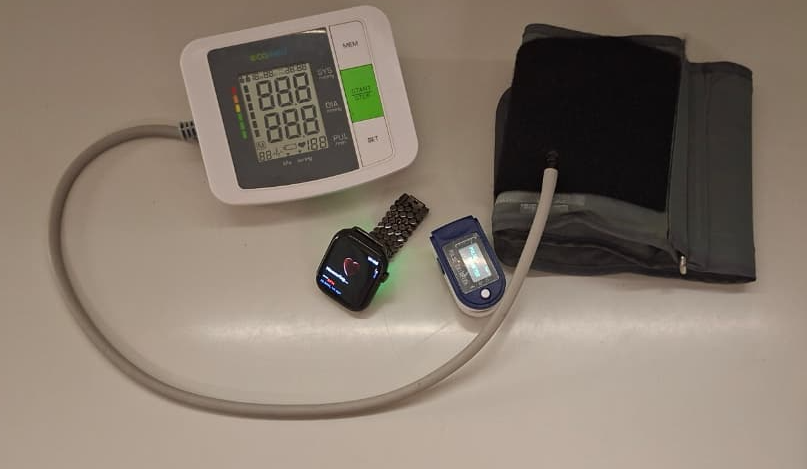
\includegraphics[width=0.9\textwidth]{FYP_Template_Spring/Figures/testing_bpe_setup.png}
    \caption{Reference devices used during the cardiovascular monitoring experiment, including a cuff-based blood-pressure monitor, an Apple Watch for heart-rate comparison, and a fingertip pulse oximeter for SpO$_2$ validation.}
    \label{fig:cardiovascular_testing_setup}
\end{figure}



\noindent For each participant and each condition, the readings from the SoleMate device and the corresponding reference devices were recorded. The absolute error was then calculated for heart rate, SpO$_2$, systolic blood pressure, and diastolic blood pressure by comparing the SoleMate output with the reference measurement. This allowed the evaluation to consider not only static resting measurements, but also the ability of the system to respond to changes in physiological state. \\


\noindent The post-activity measurements were not intended to clinically diagnose hypertension or hypotension. Instead, they were used to create a controlled variation in cardiovascular parameters and to observe whether the PPG acquisition pipeline and blood-pressure estimation model could reflect these changes. This setup provides an initial validation step for the cardiovascular monitoring subsystem before future testing on a larger and more clinically diverse population. \\


\noindent Basic hygiene precautions were followed during testing because the experiment involved skin-contact sensors and reference devices used by multiple participants. Before and after each measurement session, the contact surfaces of the SoleMate PPG sensor, the fingertip pulse oximeter, and the blood-pressure cuff were cleaned and sanitized. Participants were also asked to keep the measurement area clean and dry to improve sensor contact quality and reduce possible contamination. These precautions helped maintain a safer and much heigenic testing environment while also reducing measurement errors caused by sweat, dirt, or unstable skin contact. \\

\noindent It is important to note that the team had not yet received IRB approval at this stage of testing, which limited the ability to recruit clinical participants or conduct structured formal testing on patients with diagnosed hypertension or hypotension. As a result, the cardiovascular validation was performed informally mainly using healthy volunteers, students, and available family members. Some family participants had known blood-pressure conditions, which provided preliminary examples of abnormal or elevated readings. However, these cases were limited in number and were not evenly distributed across the dataset. Therefore, the collected data was skewed toward normal readings, with fewer hypertensive cases. For this reason, the experiment should be interpreted as an initial prototype-level validation of the sensing and estimation pipeline rather than a full clinical validation of hypertension detection. \\




\subsection{Plantar Pressure Subsystem and Ataxia Detection Model Testing}
\label{subsec:plantar_pressure_testing_setup}

\noindent The plantar-pressure subsystem was tested to verify that the sensing matrix could acquire pressure-distribution data and reconstruct it as a two-dimensional heatmap. Since the team had not yet received IRB approval during the testing period, formal testing on patients with diagnosed ataxia, multiple sclerosis, or other gait-related disorders was not conducted. Therefore, the live prototype testing was limited to validating pressure acquisition, heatmap generation, and visualization rather than clinically validating ataxia detection using real patient data. \\

\noindent Before testing, a no-load baseline was recorded from the pressure matrix to account for the resting resistance and static offsets of the sensing layer. This baseline was subtracted from the active readings so that the resulting heatmap would mainly represent applied pressure rather than fixed sensor bias. During testing, pressure was applied to different regions of the sensing surface, including areas corresponding to the heel, forefoot, and toe regions. The purpose was to check whether the high-pressure regions appeared in the expected locations on the reconstructed heatmap. \\

\noindent Additional controlled loading patterns were also tested by shifting weight toward different regions of the foot or applying uneven pressure across the sensing surface. These tests were not intended to reproduce or diagnose pathological gait patterns. Instead, they were used only to verify that the sensing matrix could reflect changes in pressure distribution and that the visualization pipeline could display these changes clearly. This distinction is important because abnormal gait patterns caused by ataxia cannot be reliably reproduced without clinical participants and proper medical validation. \\

\noindent The ataxia-detection model was therefore evaluated separately from the live prototype using available plantar-pressure heatmap data. The model-testing stage focused on assessing whether the selected machine-learning approach could classify gait-related pressure patterns using an existing dataset, while the hardware-testing stage focused on proving that the SoleMate prototype could generate usable pressure heatmaps. This separation allowed the team to validate the feasibility of both parts of the pipeline without claiming that the current prototype had been clinically tested on ataxia patients. \\

\noindent In future work, once IRB approval and clinical access are obtained, pressure data collected directly from SoleMate can be used to evaluate the complete ataxia-detection pipeline under real walking conditions. This would allow the model to be tested on data generated by the actual wearable device and compared against clinical assessment or expert-labeled gait data.





%SHOULDDD INCLUDE CALIBRATION GRAPHS AND TESTING TABLES!!


\subsection{Swelling Detection Subsystem Testing Setup}
\label{subsec:swelling_detection_testing_setup}


\noindent The swelling-detection subsystem was tested to verify that the four-flex-sensor configuration could detect controlled changes in ankle circumference and convert these changes into localized ankle-volume deviation and swelling-severity output. The purpose of this experiment was to validate the functionality of the implemented sensing and classification pipeline rather than to clinically diagnose edema. The experiment was conducted as a prototype-level informal validation using controlled circumference changes and simulated swelling conditions instead of patient-based clinical testing. \\

\noindent The final swelling-detection setup used four flex sensors arranged around the ankle in a dual-level circumferential configuration. Two flex sensors were positioned at the upper ankle measurement level, while the other two were positioned at the lower measurement level where each pair is separated by around 1.1 cm in altitude. This allowed the system to estimate two local circumferences instead of relying on a single raw deviation value. \\

\noindent Before functional testing, a calibration stage was performed to map the raw ADC readings of each flex sensor to measured circumference values. This was necessary because flex sensors measure bending and resistance variation rather than circumference directly. For each calibration point, the upper and lower ankle circumferences were measured manually using a flexible measuring tape, and the corresponding raw ADC readings from the four sensors were recorded through the Arduino Serial Monitor. Values where then mapped in order to generate the calibration curves. Four controlled configurations were used during calibration: normal, mild, moderate, and severe simulated swelling. For each sensor, a linear calibration curve of the form

\begin{equation}
    C_i = m_i R_i + b_i
\end{equation}

\noindent was generated, where $C_i$ is the estimated circumference associated with sensor $i$, $R_i$ is the raw ADC reading, and $m_i$ and $b_i$ are the slope and intercept obtained from the sensor-specific calibration curve. The two upper sensors were calibrated using the measured upper circumference, while the two lower sensors were calibrated using the measured lower circumference. This calibration step produced four separate equations, since each flex sensor had a different response depending on its placement, bending direction, soldered connection, and local contact pressure. \\

\noindent After calibration, the functional swelling test was performed by first placing the ankle-sensing assembly in the normal condition. The firmware then captured a personalized baseline volume from the normal configuration. This baseline represented the reference ankle state against which all later measurements were compared. Once the baseline was established, swelling was simulated by gradually adding controlled padding beneath the sensing region and adjusting the wrap so that the sensors remained in contact with the surface. This produced repeatable increases in measured circumference without requiring clinical participants. For each simulated swelling condition, the upper and lower circumferences were measured manually, while the Arduino output was recorded to document the raw readings, calibrated circumference estimates, calculated volume, percentage volume deviation, and final swelling classification. \\

\noindent During each test cycle, the firmware first averaged multiple ADC samples from each sensor to reduce random electrical noise. The averaged raw readings were then converted into calibrated circumference estimates using the previously obtained linear equations. The upper circumference $C_1$ was calculated as the average of the upper-left and upper-right circumference estimates, while the lower circumference $C_2$ was calculated as the average of the lower-left and lower-right circumference estimates. The monitored ankle region was then modeled as a truncated cone because the upper and lower circumferences are not necessarily equal. The resulting volume deviation was mapped to four swelling-severity classes. A deviation below $5\%$ was classified as no significant swelling, a deviation between $5\%$ and $10\%$ was classified as mild swelling, a deviation above $10\%$ and up to $30\%$ was classified as moderate swelling, and a deviation above $30\%$ was classified as severe swelling. This percentage-based approach allowed the subsystem to adapt to the user’s own baseline ankle size instead of relying on fixed raw ADC thresholds. \\

\noindent To improve the reliability of the output during testing, the firmware did not classify swelling from a single instantaneous volume reading. Instead, several volume estimates were computed and averaged to obtain a more stable current volume. The firmware also calculated a volume-spread percentage by comparing the minimum and maximum volume estimates within the same reading window. This spread value was used as an indicator of sensor-contact stability. A high spread suggested that the strap or sensors may have shifted during measurement, while a low spread indicated that the sensing contact was stable. In addition, hysteresis was applied around the severe-swelling boundary to reduce rapid switching between moderate and severe outputs when the estimated deviation was close to the $30\%$ threshold. \\



%SUMMMMM UPPPPP PARAGRAPH BUT IG BESER FE KTR REPETITION


% \noindent The testing procedure was repeated for four main configurations: no swelling, mild simulated swelling, moderate simulated swelling, and severe simulated swelling. For each configuration, the manually measured upper and lower circumferences were recorded together with the corresponding firmware outputs. This allowed the team to verify whether a controlled increase in circumference produced an increase in estimated ankle volume and whether the firmware classification followed the expected progression from no significant swelling to mild, moderate, and severe swelling. The experiment therefore validated the functional behavior of the swelling-detection subsystem, while clinical validation on patients with actual edema remains part of future work. \\






\subsection{BLE Communication and Mobile Application Testing Setup}
\label{subsec:ble_mobile_testing_setup}

\noindent This stage validated the \textbf{end-to-end BLE path}: wearable acquisition $\rightarrow$
GATT notifications $\rightarrow$ Android decryption/parsing $\rightarrow$ live UI and optional
export. Failures here are often ambiguous (stack-level disconnects, truncated ATT payloads,
descriptor races, or decrypt/format mismatches), so the procedure was designed to isolate whether
errors were introduced in \emph{transport}, \emph{cryptography}, or \emph{application parsing/UI}.
The protocol details (UUID layout, framing, and KDF) are documented in
Chapter~\ref{chapter:Implementation} (Section~\ref{sec:ble}); this subsection records what was
actually exercised during testing. \\

\noindent \textbf{Equipment and configuration.} Tests used the SoleMate Nano~33~BLE prototype, a
commercial Android smartphone with Bluetooth~5.x, and a firmware build advertising the local name
\textit{SoleMate}. Where possible, tests were repeated across multiple Android OS levels because
BLE stacks differ in permission requirements, notification delivery, and ATT MTU negotiation
behaviour. Runtime Bluetooth permissions were granted as required by the installed OS (including
\texttt{BLUETOOTH\_CONNECT} on newer releases) before attempting a connection. \\

\noindent \textbf{Connection and subscription procedure (as implemented).} The user selects the
device from \texttt{ScanActivity}; \texttt{MainActivity} then establishes a GATT connection using
the application context (to reduce connection drops when navigating to analytics screens),
performs delayed service discovery, and branches: if the Key Exchange Service is present, ECDH
public keys are exchanged and \texttt{AESCrypto} is initialised from the derived secret; otherwise
the client falls back to \texttt{initWithLegacyKeys()} for older firmware. Notifications for the
wearable characteristics are enabled through a \emph{serialized} CCCD-write queue (one characteristic
at a time). Only after this queue completes does the client request a larger ATT MTU
(\texttt{requestMtu(247)} in the implementation), because requesting MTU too early can stall
service discovery on some phones; the negotiated MTU was logged where available to confirm that
notifications were not silently truncated to the default 23-byte ATT payload. On Android~13+,
notification bytes were verified through the API's three-argument
\texttt{onCharacteristicChanged} callback (rather than relying on potentially stale
\texttt{getValue()}). \\

\noindent \textbf{Functional checks per stream.} The following GATT notification channels were
exercised: step count and motion state (IMU-derived summaries), heart rate, SpO$_2$, edema/flex
string output, plantar-pressure framed packets, and the PPG waveform characteristic. For ASCII
payload channels, decrypted strings were compared (when serial debugging was enabled) against the
Arduino Serial Monitor output to confirm that the phone matched the firmware-side plaintext prior
to encryption. For plantar pressure, the test additionally verified packet ordering and
progressive reconstruction into a complete matrix frame before heatmap rendering. For swelling,
the displayed label was checked against the firmware-reported classification string. \\

\noindent \textbf{UI and navigation.} Beyond numeric correctness, the test included navigation
through the primary monitoring screens (dashboard/readings, gait-related views, pressure matrix,
and plantar analytics) while notifications remained active, checking that secondary screens stayed
coherent with connection state (including disconnect/reconnect overlays). \\


%ADD A PIC OF APP AND SENSOR READINGS TOGETHER


\noindent Data logging and export were also included in the testing setup. After live readings were displayed in the application, the CSV export feature was tested to verify that timestamped sensor records could be generated for offline analysis. The exported files were opened after testing to check that the recorded values were formatted correctly and that the timestamps matched the measurement sequence. This step was important because exported data is required for later evaluation, documentation, and possible machine-learning analysis. \\


%ADD a diagram/ pipline


\noindent \textbf{Robustness / regression-style checks.} The same workflow was repeated under
practical stress conditions: peripheral power-cycle, app background/foreground transitions,
disconnect/reconnect, walking the phone to the edge of usable range, and rapid navigation between
activities while streaming. These checks specifically target regressions such as missed
notifications after reconnect, stale GATT callbacks after rotation, permission denials on cold
start, and truncation artefacts when ATT MTU remains low. Outcomes are summarised in
Section~\ref{subsec:ble_mobile_results}. \\



%CHECKKKKKKKKKKK
% \subsection{Full System Testing Setup}
% \label{subsec:full_system_testing_setup}






\section {Results}
% Include all the obtained results from the experiment. The results can be reported as plots, tables, charts, or any form that is relevant to your project. 

\subsection{Cardiovascular Monitoring and Blood Pressure Estimation Results}

% ------------------------------------------------------------
\subsubsection{Baseline Evaluation}
\label{subsubsec:bp_baselines}
% ------------------------------------------------------------

\noindent Before training the target architecture, six baseline models were evaluated on the same
subject-level splits to establish a performance floor and characterise the difficulty of the
task.
The baselines spanned a broad complexity range, from classical Linear Regression to a Simple
LSTM, and all received the same pre-processed three-channel input.

\begin{table}[htbp]
  \centering
  \caption{%
    Test-set performance of baseline models on the MIMIC~BP held-out subjects.
    All models were trained and evaluated on identical subject-level splits.
    Regression slope of 1.0 indicates perfect individual tracking;
    values near 0 indicate the model predicts close to the population mean.}
  \label{tab:baselines}
  \small
  \begin{tabular}{lcccccc}
    \toprule
    \multirow{2}{*}{\textbf{Model}}
      & \multicolumn{3}{c}{\textbf{SBP}}
      & \multicolumn{3}{c}{\textbf{DBP}} \\
    \cmidrule(lr){2-4}\cmidrule(lr){5-7}
      & MAE    & Slope & $r$
      & MAE    & Slope & $r$ \\
      & (mmHg) &       &
      & (mmHg) &       & \\
    \midrule
    Linear Regression & 13.69 & 0.07 & 0.24 & 8.88 & 0.10 & 0.28 \\
    Random Forest     & 13.66 & 0.11 & 0.27 & 8.96 & 0.12 & 0.29 \\
    Gradient Boosting & 13.47 & 0.11 & 0.29 & 8.78 & 0.13 & 0.32 \\
    Simple MLP        & 13.82 & 0.07 & 0.23 & 9.20 & 0.09 & 0.25 \\
    Simple LSTM       & 14.23 & 0.00 & 0.00 & 9.55 & 0.00 & 0.01 \\
    \midrule
    Simple CNN        & \textbf{12.75} & \textbf{0.20} & \textbf{0.41}
                      & \textbf{8.53}  & \textbf{0.21} & \textbf{0.43} \\
    \bottomrule
  \end{tabular}
\end{table}

\noindent SBP MAE ranged from 12.75 to 14.23\,mmHg and DBP MAE from 8.53 to 9.55\,mmHg across all
baselines.
The regression slope column reveals a consistent pattern: every model was predicting close to
the population mean, with slopes ranging from 0.00 (Simple LSTM) to 0.21 (Simple CNN), far
below the ideal value of 1.0.
The Simple CNN achieved the best overall performance and was used as the primary baseline
for comparison with the target architecture.

\begin{figure}[htbp]
    \centering
    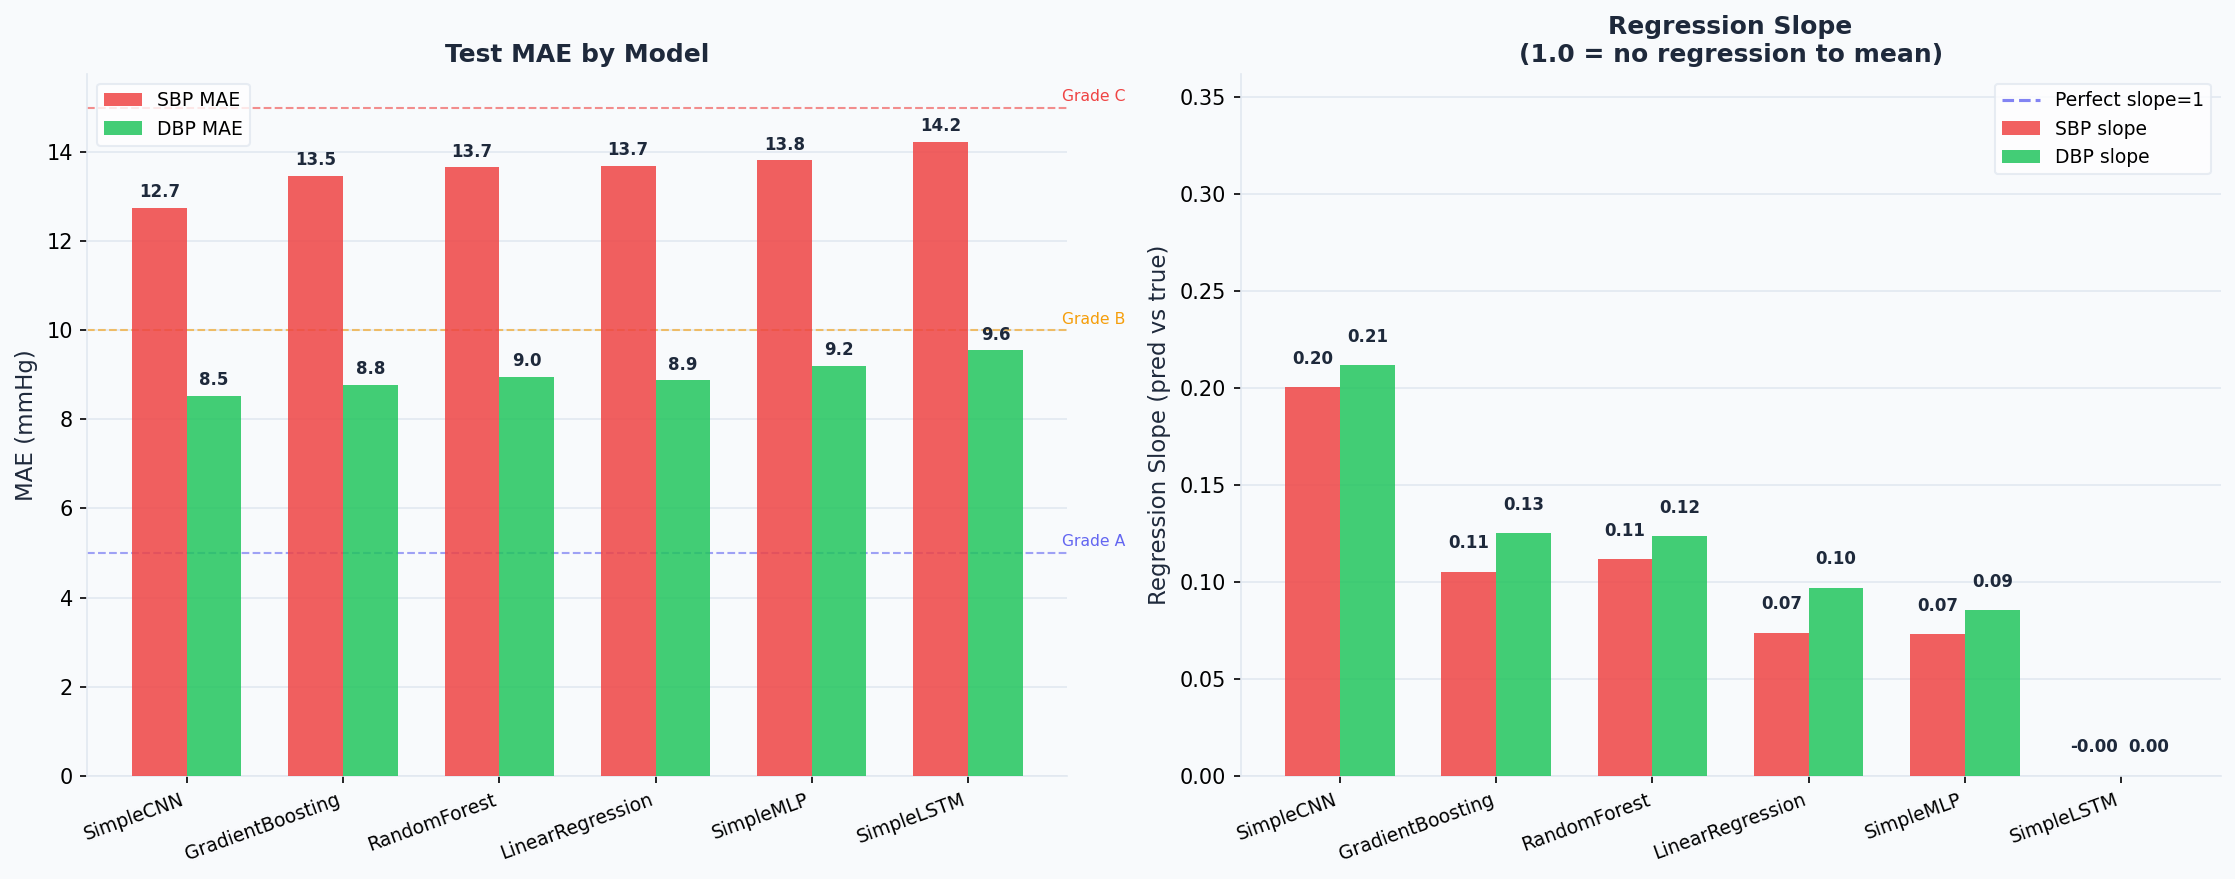
\includegraphics[width=1\textwidth]{FYP_Template_Spring/Figures/comparison_figure.png}
    \caption{Comparison of baseline model performance on the MIMIC~BP held-out subjects. The figure summarizes the SBP and DBP prediction errors across the evaluated models, showing that the Simple CNN achieved the lowest MAE and therefore served as the strongest baseline for comparison with the target blood-pressure estimation architecture.}
    \label{fig:baseline_comparison}
\end{figure}

% ------------------------------------------------------------
\subsubsection{Training Phase Results}
\label{subsubsec:bp_phase_results}
% ------------------------------------------------------------

\noindent The training curves for Phase~1 (Figure~\ref{fig:training_phase1}) confirm that both SBP
and DBP validation MAE were still declining at the early-stopping point (epoch~40, best at
epoch~25), justifying the transition to Adam in Phase~2.

\begin{figure}[H]
    \centering
    \begin{minipage}{0.95\linewidth}
        \centering
        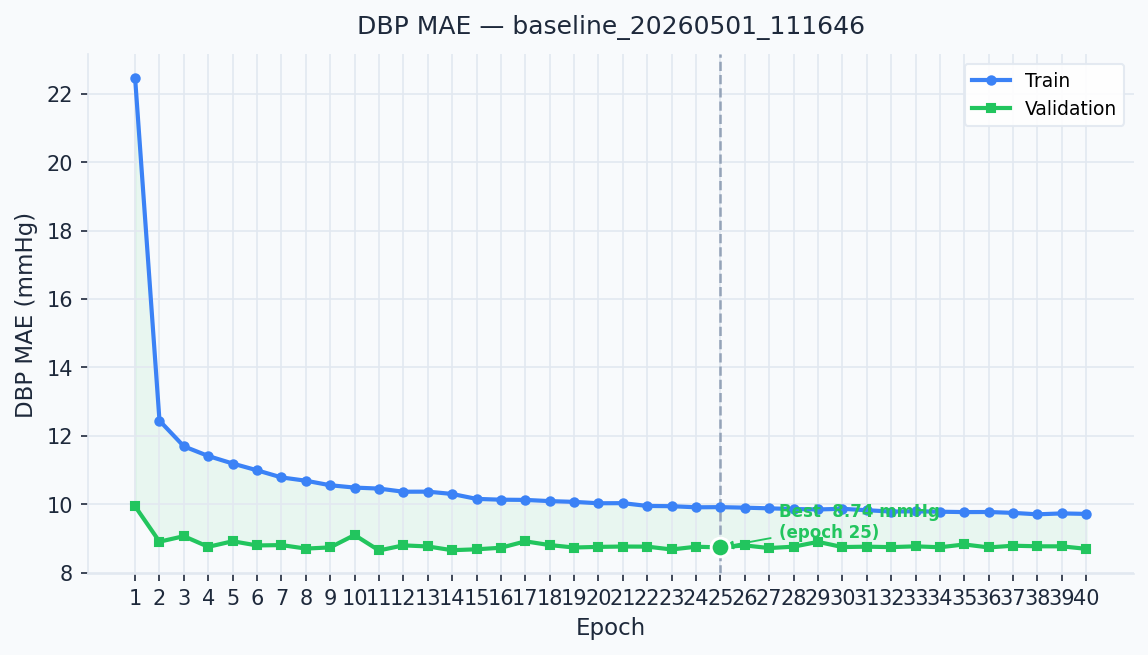
\includegraphics[width=\linewidth]{Figures/3_train_val_dbp.png}
        \caption*{(a) DBP MAE training and validation curves.}
    \end{minipage}
    \vspace{0.7cm}
    \begin{minipage}{0.95\linewidth}
        \centering
        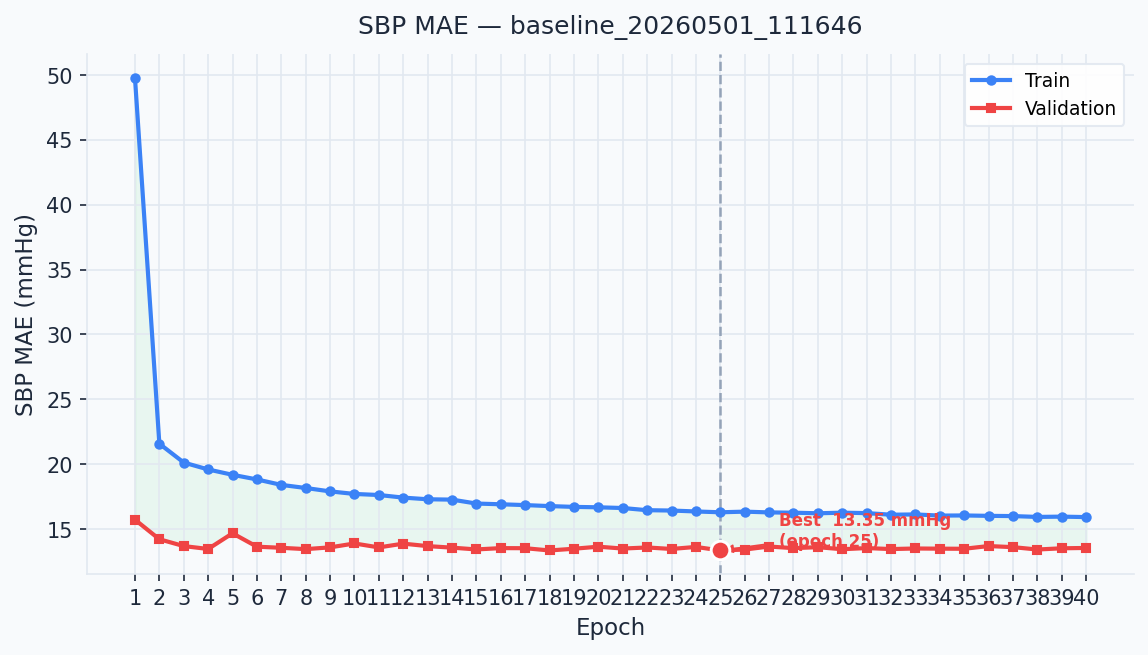
\includegraphics[width=\linewidth]{Figures/2_train_val_sbp.png}
        \caption*{(b) SBP MAE training and validation curves.}
    \end{minipage}
    \caption{Phase~1 training history (RMSprop, $\mathrm{lr}{=}10^{-4}$). Both validation
    curves were still declining at the early-stopping point, indicating premature termination.}
    \label{fig:training_phase1}
\end{figure}

\noindent The top 8 configurations from the Phase~3 grid search are reported in
Table~\ref{tab:gridsearch}.
Validation MAEs across all 24 runs ranged narrowly from 10.71 to 11.01\,mmHg — a spread of
only 0.30\,mmHg — indicating that the model reached a performance plateau largely independent
of hyperparameter choice.
The best configuration (RMSprop, $\mathrm{lr}{=}10^{-3}$, batch size~128,
weight decay $10^{-4}$, best at epoch~34) was selected as the final model.

\begin{table}[htbp]
  \centering
  \caption{%
    Top 8 of 24 grid search configurations by validation MAE.
    The \textbf{bold} row indicates the selected configuration.
    LR = learning rate; BS = batch size; WD = weight decay.}
  \label{tab:gridsearch}
  \small
  \begin{tabular}{llcccccc}
    \toprule
    \textbf{Opt.} & \textbf{LR} & \textbf{BS} & \textbf{WD}
      & \textbf{Best Ep.} & \textbf{Val MAE}
      & \textbf{SBP MAE} & \textbf{DBP MAE} \\
    & & & & & (mmHg) & (mmHg) & (mmHg) \\
    \midrule
    \textbf{RMSprop} & $\mathbf{10^{-3}}$ & \textbf{128} & $\mathbf{10^{-4}}$
      & \textbf{34} & \textbf{10.71} & \textbf{12.80} & \textbf{8.18} \\
    Adam    & $10^{-3}$ & 128 & $10^{-4}$ & 26 & 10.78 & 12.87 & 8.17 \\
    RMSprop & $10^{-3}$ & 128 & $10^{-3}$ & 20 & 10.77 & 12.63 & 8.71 \\
    Adam    & $10^{-3}$ & 256 & $10^{-4}$ & 15 & 10.84 & 12.67 & 8.45 \\
    RMSprop & $3{\times}10^{-4}$ & 128 & $10^{-4}$ & 24 & 10.84 & 12.85 & 8.09 \\
    Adam    & $10^{-3}$ & 128 & $10^{-3}$ & 12 & 10.86 & 12.66 & 8.74 \\
    Adam    & $10^{-4}$ & 128 & $10^{-4}$ & 14 & 10.88 & 12.87 & 8.58 \\
    RMSprop & $10^{-4}$ & 128 & $10^{-3}$ & 18 & 10.88 & 12.73 & 8.64 \\
    \bottomrule
  \end{tabular}
\end{table}

\noindent Table~\ref{tab:final_results} summarises test-set performance across all three training phases
alongside the best simple baseline and the published reference result.

\begin{table}[htbp]
  \centering
  \caption{%
    Test-set performance across all training phases compared to the best simple baseline and
    the reference result of Slap\-ni\v{c}ar et al.\ \cite{Slapnicar2019}.
    Overall MAE is the arithmetic mean of SBP and DBP MAE.
    $^\dagger$Slap\-ni\v{c}ar et al.\ used LOSO on MIMIC-III (a strictly harder protocol);
    all other rows use a fixed subject-level split on MIMIC~BP.
    The best value in each column (excluding the reference row) is shown in \textbf{bold}.}
  \label{tab:final_results}
  \begin{tabular}{p{4.5cm}ccc}
    \toprule
    \textbf{Configuration} & \textbf{SBP MAE} & \textbf{DBP MAE} & \textbf{Overall MAE} \\
    & (mmHg) & (mmHg) & (mmHg) \\
    \midrule
    Slap\-ni\v{c}ar et al.\ (PPG+PPG$'$+PPG$''$, no pers.)$^\dagger$
      & 15.41 & 12.38 & 13.90 \\
    \midrule
    Best Baseline (Simple CNN)
      & \textbf{12.75} & 8.53 & 10.64 \\
    \midrule
    Phase 1: RMSprop, $\mathrm{lr}=10^{-4}$  & 13.08 & 8.67 & 10.88 \\
    Phase 2: Adam, $\mathrm{lr}=10^{-4}$     & 12.97 & 8.61 & 10.79 \\
    Phase 3: Best Grid Config                 & 12.80 & \textbf{8.18} & \textbf{10.49} \\
    \bottomrule
  \end{tabular}
\end{table}

\noindent The iterative refinement produced a consistent reduction in overall MAE from
10.88\,mmHg (Phase~1) to 10.49\,mmHg (Phase~3).
Phases~1 and~2 both fell short of the Simple CNN baseline (10.64\,mmHg); only the
grid-searched Phase~3 configuration surpassed it, driven primarily by improved DBP estimation
(8.18 vs.\ 8.53\,mmHg).
The training history of the final model is shown in Figure~\ref{fig:training_final}.

\begin{figure}[H]
    \centering
    \begin{minipage}{0.95\linewidth}
        \centering
        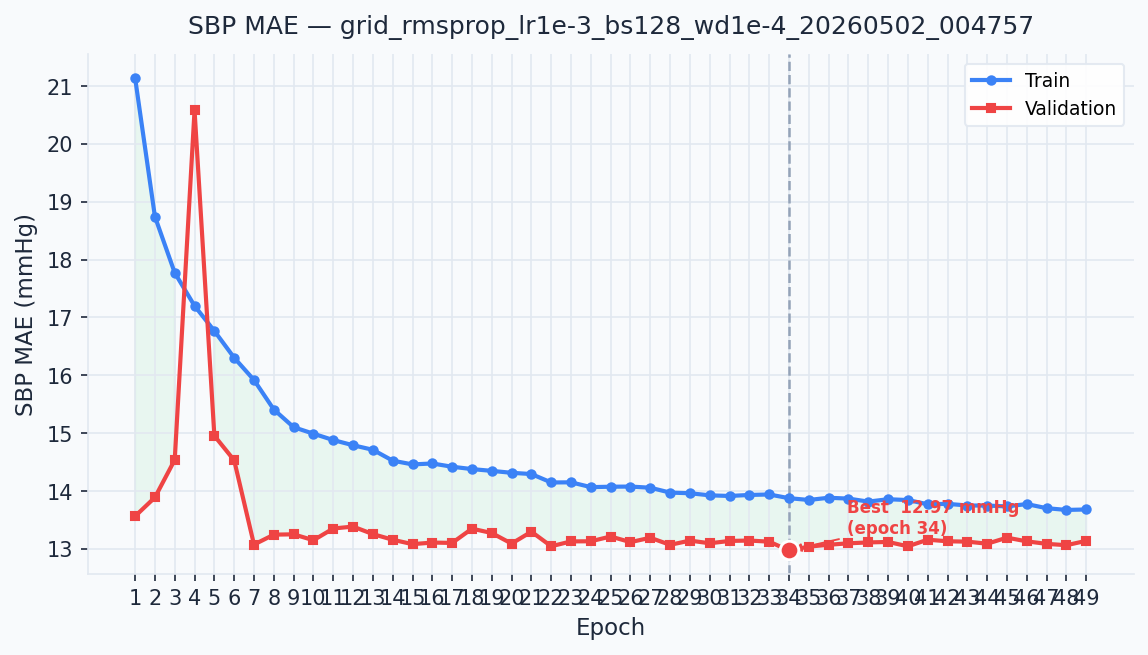
\includegraphics[width=\linewidth]{FYP_Template_Spring/Figures/2_train_val_sbp_best.png}
        \caption*{(a) SBP MAE training and validation curves.}
    \end{minipage}
    \vspace{0.4cm}
    \begin{minipage}{0.95\linewidth}
        \centering
        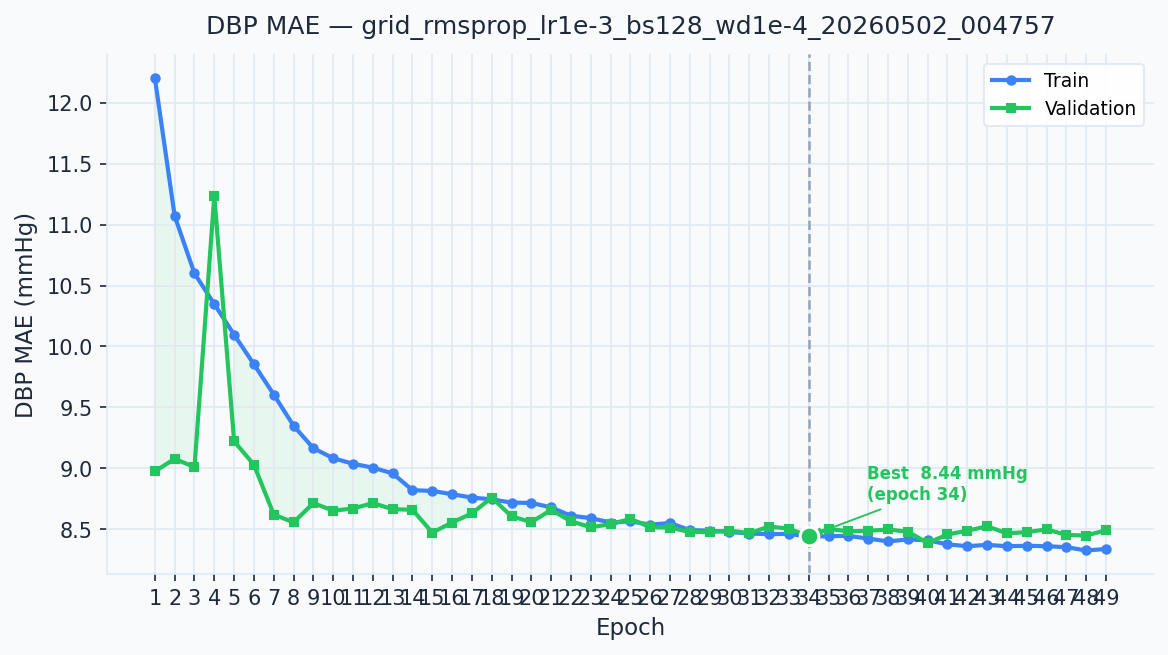
\includegraphics[width=\linewidth]{FYP_Template_Spring/Figures/3_train_val_dbp_best.png}
        \caption*{(b) DBP MAE training and validation curves.}
    \end{minipage}
    \caption{Training history for the final model (RMSprop, $\mathrm{lr}{=}10^{-3}$,
    batch size~128, weight decay~$10^{-4}$, best at epoch~34).}
    \label{fig:training_final}
\end{figure}

\subsection{Plantar Pressure Subsystem and Ataxia Detection Model Results}
\label{subsec:plantar_pressure_ataxia_results}
% ------------------------------------------------------------
\subsubsection{Discussion}
\label{subsubsec:interpretation}
% ------------------------------------------------------------

\noindent Across all 24 grid search experiments and all six baseline models, SBP MAE consistently
settled in the range 12.6--14.2\,mmHg and DBP MAE in the range 8.1--9.6\,mmHg, regardless
of optimiser, learning rate, batch size, or model family.
This saturation reflects a structural constraint of calibration-free cross-subject estimation
rather than a deficiency in implementation.
PPG waveform morphology encodes physiological correlates of blood pressure changes
\emph{within} a subject; however, the absolute baseline pressure of an unseen subject is
determined by long-term vascular properties that are invisible to the PPG sensor.
A model trained without per-subject calibration data is therefore forced to predict near the
population mean for each new individual, which explains the near-zero regression slopes
observed across all model families (Table~\ref{tab:baselines}). \\

\noindent The final overall MAE of 10.49\,mmHg is lower than the 13.90\,mmHg reported by
Slap\-ni\v{c}ar et al.\ for the equivalent no-personalisation, three-channel configuration.
Two methodological differences account for this gap: their evaluation used a strictly harder
leave-one-subject-out (LOSO) protocol in which every test subject is completely excluded from
training, whereas this work uses a fixed subject-level split; and training was performed on
MIMIC~BP rather than raw MIMIC-III, whose tighter quality controls yield cleaner label
alignment.
These differences mean the numerical comparison is not direct.
What the comparison does confirm is that the re-implemented architecture behaves
consistently with the published baseline: both reproduce the well-documented phenomenon
of calibration-free models converging toward the population mean, and both reach similar
error magnitudes under their respective evaluation conditions.
Slap\-ni\v{c}ar et al.\ explicitly identify this as the fundamental limitation of
no-personalisation PPG-based estimation~\cite{Slapnicar2019}, and the results here align
with that characterisation. \\

\noindent Under the British Hypertension Society (BHS) grading protocol, the final model achieves
\textbf{Grade~C} for SBP (MAE $<$\,15\,mmHg) and approaches \textbf{Grade~B} for DBP
(MAE $<$\,10\,mmHg), consistent with published performance ranges for calibration-free,
cross-subject PPG-based estimation without personalisation~\cite{Slapnicar2019}.
This system is therefore best understood as a \textbf{proof of concept}: it demonstrates
that the SpectroTemporalNet architecture can be re-implemented, trained end-to-end on a
more diversified dataset collected from non ICU population, and deployed on-device via ExecuTorch within the application.
Reaching clinically meaningful accuracy requires the additions outlined below.


% ------------------------------------------------------------
\subsubsection{Limitations}
\label{subsubsec:limitations}
% ------------------------------------------------------------

\paragraph{Calibration-free cross-subject generalisation.}
Without a subject-specific reference measurement, the PPG waveform alone cannot resolve
between-subject BP offsets.
The near-zero regression slopes observed across all model families (Table~\ref{tab:baselines})
confirm that the models are estimating a fixed population-level value rather than tracking
individual variation.
This is a known constraint of the calibration-free paradigm, documented in the original
paper~\cite{Slapnicar2019} and reproduced here as expected.

\paragraph{Dataset scope.}
MIMIC~BP is derived exclusively from ICU recordings, which over-represent haemodynamically
unstable patients and under-represent the healthy adult population that SoleMate targets.
Training on a more diverse, community-collected dataset would reduce the population mismatch
and likely improve generalisation to everyday users.

\paragraph{Model capacity.}
The grid search demonstrated that validation MAE varied by only 0.30\,mmHg across all 24
configurations, indicating that the current performance ceiling is not attributable to
hyperparameter choice or model capacity.
Scaling the architecture without a commensurate increase in subject diversity would risk
overfitting to the training distribution without improving cross-subject generalisation.


% ------------------------------------------------------------
\subsubsection{Future Work}
\label{subsubsec:future_work}
% ------------------------------------------------------------

\paragraph{Subject-specific personalisation.}
The most impactful near-term improvement is the integration of subject-specific calibration.
Slap\-ni\v{c}ar et al.\ report that incorporating just 20\,\% of a subject's own recordings
reduces SBP MAE from 15.41 to 9.43\,mmHg and DBP MAE from 12.38 to 6.88\,mmHg under
LOSO evaluation~\cite{Slapnicar2019} — improvements of 39\,\% and 44\,\% respectively. A testing script implementing this
fine-tuning workflow; integrating it into the deployed system would require pairing the
application with a Bluetooth sphygmomanometer to acquire one or more reference cuff
measurements per user.

\paragraph{Expanded and more representative training data.}
Collecting or incorporating multi-centre, non-ICU PPG datasets would directly address the
population mismatch identified above.
Community-collected data spanning a wider range of ages, fitness levels, and cardiovascular
conditions would improve the model's ability to generalise to the everyday users SoleMate is
designed for.

\paragraph{Architectural improvements.}
More expressive encoders — transformer-based temporal attention, multi-scale feature pyramids,
or contrastive pre-training on large unlabelled PPG corpora — have shown incremental gains in
related work and represent a natural evolution of the current architecture.
These improvements should be pursued in parallel with data expansion rather than in isolation,
as architectural capacity and training data diversity are complementary requirements for
meaningful generalisation gains.

\subsection{Swelling Detection Subsystem Results}
\label{subsec:swelling_detection_results}

\subsection{BLE Communication and Mobile Application Results}
\label{subsec:ble_mobile_results}


%CHECKKKKKK
% \subsection{Overall Prototype-Level Validation Summary}
% \label{subsec:overall_prototype_validation_summary}

\section{Discussions and Future Work}
\subsection{Discussion of Cardiovascular Monitoring Results}
\label{subsec:discussion_cardiovascular}



\subsection{Discussion of Plantar Pressure and Ataxia Detection Results}
\label{subsec:discussion_plantar_pressure_ataxia}

\subsection{Discussion of Swelling Detection Results}
\label{subsec:discussion_swelling}

\subsection{Discussion of BLE Communication and Mobile Application Results}
\label{subsec:discussion_ble_mobile}

\subsection{System Limitations}
\label{subsec:system_limitations}


\subsection{Future Work}
\label{subsec:future_work}

